\documentclass[xcolor=dvipsnames]{beamer}

\usepackage[utf8]{inputenc}
\usepackage{multicol}
\usepackage{amssymb,amsmath,amsbsy,cmath} 
\usepackage{bm}    
\usepackage{graphicx,graphics,xcolor}
\usepackage{xcolor}
\usepackage{physics}
\usepackage{comment}
\usepackage{caption}
\usepackage[style=authortitle,backend=bibtex]{biblatex}
\addbibresource{References.bib}
\usepackage{yfonts}
\usepackage{pifont}


\newcommand\blfootnote[1]{%
  \begingroup
  \renewcommand\thefootnote{}\footcite{#1}%
  \addtocounter{footnote}{-1}%
  \endgroup
}


\usetheme{Madrid}
\useoutertheme{miniframes} % Alternatively: miniframes, infolines, split
\useinnertheme{circles}


\title[Schwarzschild geometry]{Schwarzschild Geometry: Metric}
\date{\today}
\author[Universidad del Valle]{Nicolle Tello}
\institute[]{Universidad del Valle \\ Departamento de física}

\begin{document}
	
	\begin{frame}[plain]
		\titlepage
	\end{frame}
	
	\begin{frame}{Table of contents}
    \tableofcontents
	\end{frame}
	
%------------------------------------	
\section{Introduction}	
	\begin{frame}{Introduction}
	the Schwarzschild metric is the most general spherically symmetric vacuum solution of the Einstein field equations
	    \begin{figure}
    \centering
    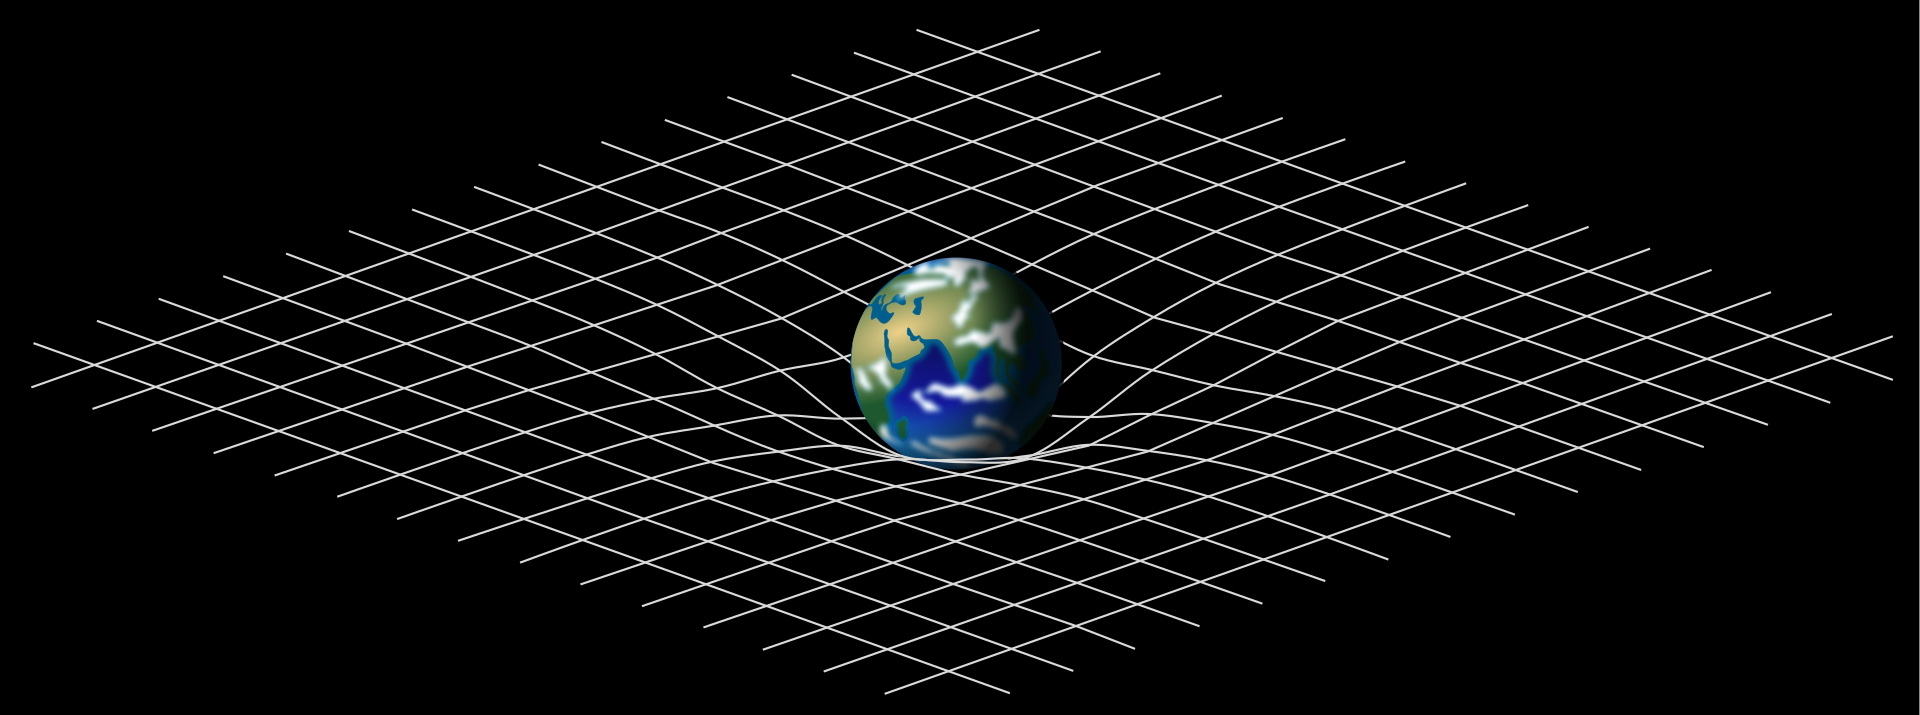
\includegraphics[width=0.9\textwidth]{Presentations/Images/1_Spacetime_lattice_analogy.svg.png}
\end{figure}
\let\thefootnote\relax\footnote{\tiny By Mysid - Own work. Self -made in Blender &amp; Inkscape., CC BY-SA 3.0,  \\ \hspace{0.25in}\url{https://commons.wikimedia.org/w/index.php?curid=45121761} }
	\end{frame}
\section{The general static isotropic metric.}

    
\begin{frame}{Static spacetime}
To construct the most general metric for a static spatially isotropic spacetime, we start with the line element:
$$ds^2=g_{\mu\nu}dx^{\mu}dx^{\nu}$$
    \begin{block}{Properties of a static spacetime}
    \begin{enumerate}
        \item\label{indt} All the metric components are independent of $x^0$.
        \item The line element is invariant under $x^0 \rightarrow -x^0$
    \end{enumerate}
    \end{block}
    \begin{exampleblock}{}
    If the spacetime only satisfies \ref{indt}, it's called \textbf{stationary}
    \end{exampleblock}
\end{frame}

\begin{frame}{To get an isotropic metric}
\begin{multicols}{2}
    \begin{column}{0.46\textwidth}
    \begin{block}{\centering Isotropic metric}
    \centering
    It's obtained when $ds^2$ depends only on rotational invariants of $x^i$ and $dx^i$
    \end{block}
    \end{column}
    
    \begin{column}{0.48\textwidth}
    \begin{exampleblock}
    {}\centering The only rotational invariants and their differentials:
    $$\vec{x} \cdot \vec{x}, \quad d \vec{x} \cdot d \vec{x}, \quad \vec{x} \cdot d \vec{x}$$
    \end{exampleblock}
    \end{column}
\end{multicols}
    
    \begin{block}
    {} Starting with the most general form of a spatially isotropic metric
    $$ds^2=A(t,r)dt^2-B(t,r)dt\Vec{x}\cdot d\Vec{x} -C(t,r)(\Vec{x}\cdot d\Vec{x})^2-D(t,r)d\Vec{x}^2$$
    \end{block}
\end{frame}

\begin{frame}{To get an isotropic metric}
\begin{exampleblock}
{}Transforming to spherical polar coordinates, we get:
    $$
\vec{x} \cdot \vec{x}=r^{2}, \quad \vec{x} \cdot d \vec{x}=r d r, \quad d \vec{x} \cdot d \vec{x}=d r^{2}+r^{2} d \theta^{2}+r^{2} \sin ^{2} \theta d \phi^{2}
$$
\end{exampleblock}
Then, the metric takes the form:
$$
\begin{aligned}
d s^{2}=& A(t, r) d t^{2}-B(t, r) r d t d r-C(t, r) r^{2} d r^{2} \\
&-D(t, r)\left(d r^{2}+r^{2} d \theta^{2}+r^{2} \sin ^{2} \theta d \phi^{2}\right)
\end{aligned},
$$
where it can also be written as
$$
d s^{2}=A(t, r) d t^{2}-B(t, r) d t d r-C(t, r) d r^{2}-D(t, r)\left(d \theta^{2}+\sin ^{2} \theta d \phi^{2}\right)
$$
\end{frame}
\begin{frame}{To get an isotropic metric}
    However, we can express it in terms of a new radial coordinate
    $$
d s^{2}=A(t, \bar{r}) d t^{2}-B(t, \bar{r}) d t d \bar{r}-C(t, \bar{r}) d \bar{r}^{2}-\bar{r}^{2}\left(d \theta^{2}+\sin ^{2} \theta d \phi^{2}\right)
$$
\begin{block}
{Introducing a new timelike coordinate.}
Using
$$
d \bar{t}=\Phi(t, \bar{r})\left[A(t, \bar{r}) d t-\frac{1}{2} B(t, \bar{r}) d \bar{r}\right]
$$
we can find
$$
A d t^{2}-B d t d \bar{r}=\frac{1}{A \Phi^{2}} d \bar{t}^{2}-\frac{B}{4 A} d \bar{r}^{2}
$$
and redefine the functions $A$ and $B$
\end{block}
\end{frame}
\begin{frame}{To get an isotropic metric}
    The functions take the new form
    $$
\bar{A}=1 /\left(A \Phi^{2}\right) \text { and } \bar{B}=C+B /(4 A)
$$
from which we get the isotropic metric
\begin{block}
{}$$
d s^{2}=A(t, r) d t^{2}-B(t, r) d r^{2}-r^{2}\left(d \theta^{2}+\sin ^{2} \theta d \phi^{2}\right)
$$

\end{block}
\end{frame}

\begin{frame}{The stationary isotropic metric}
    To get the form of the metric for a general static spatially isotropic spacetime, we need the metric functions to be independent of the timelike coordinate. This means:
    \begin{block}
    {}$$
d s^{2}=A(t, r) d t^{2}-B(t, r) d r^{2}-r^{2}\left(d \theta^{2}+\sin ^{2} \theta d \phi^{2}\right)
$$
    \end{block}
    \begin{figure}
        \centering
        
\includegraphics[width=0.05\textwidth]{Presentations/Images/1_da.png}
    \end{figure}
    \begin{block}
    {}$$
d s^{2}=A( r) d t^{2}-B(r) d r^{2}-r^{2}\left(d \theta^{2}+\sin ^{2} \theta d \phi^{2}\right)
$$
    \end{block}
\end{frame}
%---------------------------------------------------------------------------------------------
\section{The empty-space field equations}
\begin{frame}{Solving the empty-space field equations}
To solve the empty-space field equations, we must have a Ricci tensor that vanishes. This is:
    $$
R_{\mu \nu}=\partial_{\nu} \Gamma_{\mu \sigma}^{\sigma}-\partial_{\sigma} \Gamma_{\mu \nu}^{\sigma}+\Gamma_{\mu \sigma}^{\rho} \Gamma_{\rho \nu}^{\sigma}-\Gamma_{\mu \nu}^{\rho} \Gamma_{\rho \sigma}^{\sigma}=0
$$
having in mind that
$$
\Gamma_{\mu \nu}^{\sigma}=\frac{1}{2} g^{\sigma \rho}\left(\partial_{\nu} g_{\rho \mu}+\partial_{\mu} g_{\rho \nu}-\partial_{\rho} g_{\mu \nu}\right)
$$
To solve this, we start with the non-zero elements of the metric $g_{\mu\nu}$
  $$
\begin{array}{ll}
g_{00}=A(r), & g^{00}=1 / A(r) \\
g_{11}=-B(r), & g^{11}=-1 / B(r) \\
g_{22}=-r^{2}, & g^{22}=-1 / r^{2} \\
g_{33}=-r^{2} \sin ^{2} \theta, & g^{33}=-1 /\left(r^{2} \sin ^{2} \theta\right)
\end{array}
$$
\end{frame}

\begin{frame}{Solving the empty-space field equations}
The connections coeffients are found as shown
 \small
$$
\begin{aligned}
&\Gamma_{00}^{0}=0\\
&\Gamma_{00}^{i}=-\frac{1}{2} g^{i \rho} \partial_{\rho} g_{00} \quad & \Rightarrow & \quad \Gamma_{00}^{1}=\frac{1}{2 B(r)} \frac{d A(r)}{d r}\\
&\Gamma_{0 i}^{0}=\frac{1}{2} g^{0 \rho}\left(\partial_{i} g_{\rho 0}+\partial_{0} g_{\rho i}-\partial_{\rho} g_{0 i}\right)=\frac{1}{2} g^{00} \partial_{i} g_{00} \quad & \Rightarrow & \quad \Gamma_{01}^{0}=\frac{1}{2 A(r)} \frac{d A(r)}{d r}\\
&\Gamma_{i j}^{0}=0\\
&\Gamma_{i i}^{i}=\frac{1}{2} g^{i \rho}\left(\partial_{i} g_{\rho i}+\partial_{i} g_{\rho i}-\partial_{\rho} g_{i i}\right)=\frac{1}{2} g^{i i} \partial_{i} g_{i i} \quad & \Rightarrow & \quad \Gamma_{11}^{1}=\frac{1}{2 B(r)} \frac{d B(r)}{d r}\\
&\Gamma_{22}^{1}=\frac{1}{2} g^{11}\left(\partial_{2} g_{12}+\partial_{2} g_{12}-\partial_{1} g_{22}\right) \quad & \Rightarrow & \quad \Gamma_{22}^{1}=-\frac{r}{B(r)}\\
&\Gamma_{33}^{1}=-\frac{1}{2} g^{11} \partial_{1} g_{33} \quad & \Rightarrow & \quad \Gamma_{33}^{1}=-\frac{r \sin ^{2} \theta}{B(r)}\\
\end{aligned}
$$
\end{frame}

\begin{frame}{Solving the empty-space field equations}
Only nine of the connection coefficients are non-zero:
\begin{block}
{}  
$$
\begin{array}{lll}
\Gamma_{01}^{0}=A^{\prime} /(2 A), & \Gamma_{00}^{1}=A^{\prime} /(2 B), & \Gamma_{11}^{1}=B^{\prime} /(2 B) \\
\Gamma_{22}^{1}=-r / B, & \Gamma_{33}^{1}=-\left(r \sin ^{2} \theta\right) / B, & \Gamma_{12}^{2}=1 / r \\
\Gamma_{33}^{2}=-\sin \theta \cos \theta, & \Gamma_{13}^{3}=1 / r, & \Gamma_{23}^{3}=\cot \theta
\end{array}
$$
\end{block}
We'll use these to get Ricci's tensor  
\end{frame}

\begin{frame}{Solving the empty-space field equations}
\begin{block}
{Diagonal components of the Ricci tensor}
$$
\begin{aligned}
&R_{00}=-\frac{A^{\prime \prime}}{2 B}+\frac{A^{\prime}}{4 B}\left(\frac{A^{\prime}}{A}+\frac{B^{\prime}}{B}\right)-\frac{A^{\prime}}{r B} \\
&R_{11}=\frac{A^{\prime \prime}}{2 A}-\frac{A^{\prime}}{4 A}\left(\frac{A^{\prime}}{A}+\frac{B^{\prime}}{B}\right)-\frac{B^{\prime}}{r B} \\
&R_{22}=\frac{1}{B}-1+\frac{r}{2 B}\left(\frac{A^{\prime}}{A}-\frac{B^{\prime}}{B}\right) \\
&R_{33}=R_{22} \sin ^{2} \theta
\end{aligned}
$$
\end{block}
\end{frame}

\begin{frame}{Solving the empty-space field equations}
Since the tensor must vanish, we can get the relationship
    $$
A^{\prime} B+A B^{\prime}=0
$$
Showing that $AB=constant$, so we can use $B=\alpha/A \rightarrow A+rA'=\alpha$
$$
\frac{d(r A)}{d r}=\alpha
$$
Integrating, we get
$$
A(r)=\alpha\left(1+\frac{k}{r}\right) \quad \text { and } \quad B(r)=\left(1+\frac{k}{r}\right)^{-1}
$$
\end{frame}
\begin{frame}{Solving the empty-space field equations}
    We can get the constants $k$ and $\alpha$ for a spherically symmetric mass $M$ as:
    $$k=-\frac{2GM}{c^2}\quad \text{and}\quad \alpha= c^2$$
    \begin{block}{Schwarzschild metric for the empty spacetime outside a spherical body of mass M}
    $$d s^{2}=c^{2}\left(1-\frac{2 G M}{c^{2} r}\right) d t^{2}-\left(1-\frac{2 G M}{c^{2} r}\right)^{-1} d r^{2}-r^{2} d \theta^{2}-r^{2} \sin ^{2} \theta d \phi^{2}$$
    \end{block}
\end{frame}
\begin{frame}{Birkhoff's theorem}
For a non-stationary metric
    $$
d s^{2}=A(t, r) d t^{2}-B(t, r) d r^{2}-r^{2}\left(d \theta^{2}+\sin ^{2} \theta d \phi^{2}\right)
$$
but solving the Einstein's empty space field equations $R_{\mu \nu}=0$ with this expression leads to the same metric
\begin{block}{Birkhoff's theorem}
\textit{The spacetime geometry outside a general
spherically symmetric matter distribution is the Schwarzschild geometry}
\end{block}
\end{frame}
%-----------------------------------------------------------------------------
\section{Example: Gravitational redshift}
\begin{frame}{Emision and receptions of two light signals}
    \begin{figure}
        \centering
        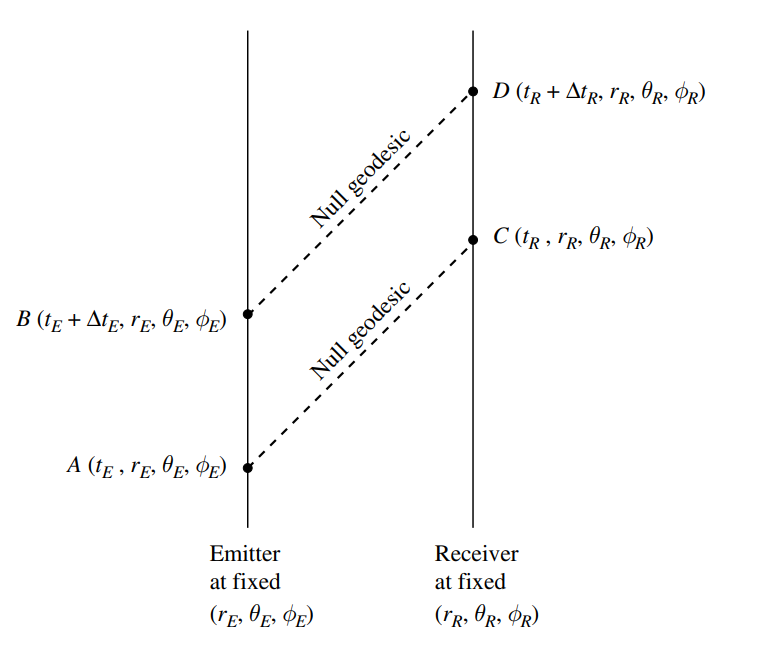
\includegraphics[width=0.7\textwidth]{Presentations/Images/1_rs.png}
        
    
    \end{figure}
\end{frame}
\begin{frame}{Gravitational redshift in a null curve}
In a null curve $ds^2=0$ at all points. This means
$$
c^{2}\left(1-\frac{2 \mu}{r}\right) d t^{2}=\left(1-\frac{2 \mu}{r}\right)^{-1} d r^{2}+r^{2} d \theta^{2}+r^{2} \sin ^{2} \theta d \phi^{2}
$$
using an affine parameter $\sigma$
$$
\frac{d t}{d \sigma}=\frac{1}{c}\left(1-\frac{2 \mu}{r}\right)^{-1 / 2}\left[-g_{i j} \frac{d x^{i}}{d \sigma} \frac{d x^{j}}{d \sigma}\right]^{1 / 2}
$$
and integrating
$$
t_{R}-t_{E}=\frac{1}{c} \int_{\sigma_{E}}^{\sigma_{R}}\left(1-\frac{2 \mu}{r}\right)^{-1 / 2}\left[-g_{i j} \frac{d x^{i}}{d \sigma} \frac{d x^{j}}{d \sigma}\right]^{1 / 2} d \sigma
$$
\end{frame}
\begin{frame}{}
    But we have that $\Delta t_{R}=\Delta t_{E}$ and $d r=d \theta=d \phi=0$, then:
    $$
c^{2} d \tau^{2} \equiv d s^{2}=c^{2}\left(1-\frac{2 \mu}{r}\right) d t^{2}
$$
and since $r$ is constant, we can integrate to obtain
$$\Delta \tau_{E}=\left(1-\frac{2 \mu}{r_{E}}\right)^{1 / 2} \Delta t_{E} \quad \text{and} \quad \Delta \tau_{R}=\left(1-\frac{2 \mu}{r_{R}}\right)^{1 / 2} \Delta t_{R}$$
which leads to 
$$
\frac{\Delta \tau_{R}}{\Delta \tau_{E}}=\left(\frac{1-2 \mu / r_{R}}{1-2 \mu / r_{E}}\right)^{1 / 2}
$$
that is the basis of the formula for the gravitational redshift
\end{frame}
\begin{frame}{}
The frequencies of the photon follow the relation
    $$
\frac{\nu_{R}}{\nu_{E}}=\left[\frac{1-2 G M /\left(r_{E} c^{2}\right)}{1-2 G M /\left(r_{R} c^{2}\right)}\right]^{1 / 2}
$$
This can be generalized as
$$
d s^{2}=g_{00}(\vec{x}) d t^{2}+g_{i j}(\vec{x}) d x^{i} d x^{j}
$$
where we find that
$$
\frac{\nu_{R}}{v_{E}}=\left[\frac{g_{00}\left(\vec{x}_{E}\right)}{g_{00}\left(\vec{x}_{R}\right)}\right]^{1 / 2}
$$
\end{frame}
\section{}
\begin{frame}[plain]
    \centering
    \Huge Thanks for your attention
\end{frame}
\end{document}